
\section{AIG CDS data over 2005 - 2010}
\label{sec:aig-cds-data}

\subsection{The data dynamic}
\label{sec:data-dynamic}



In this section we will apply the previous results on datas provided by AIG.

In the paper \cite{OTRATS}, A.cousin \& I.Niang showed that the CDS market contains
no  arbitration   opportunity  if   credit  curve   is  a   default  distribution
function witch implied that this function must be a decreasing function.\\
Among  the period  16/08/2005 -  28/09/2007  we can  see that  the credit  curve
appears to be non decreasing :

\begin{figure}[H]
  \centering
  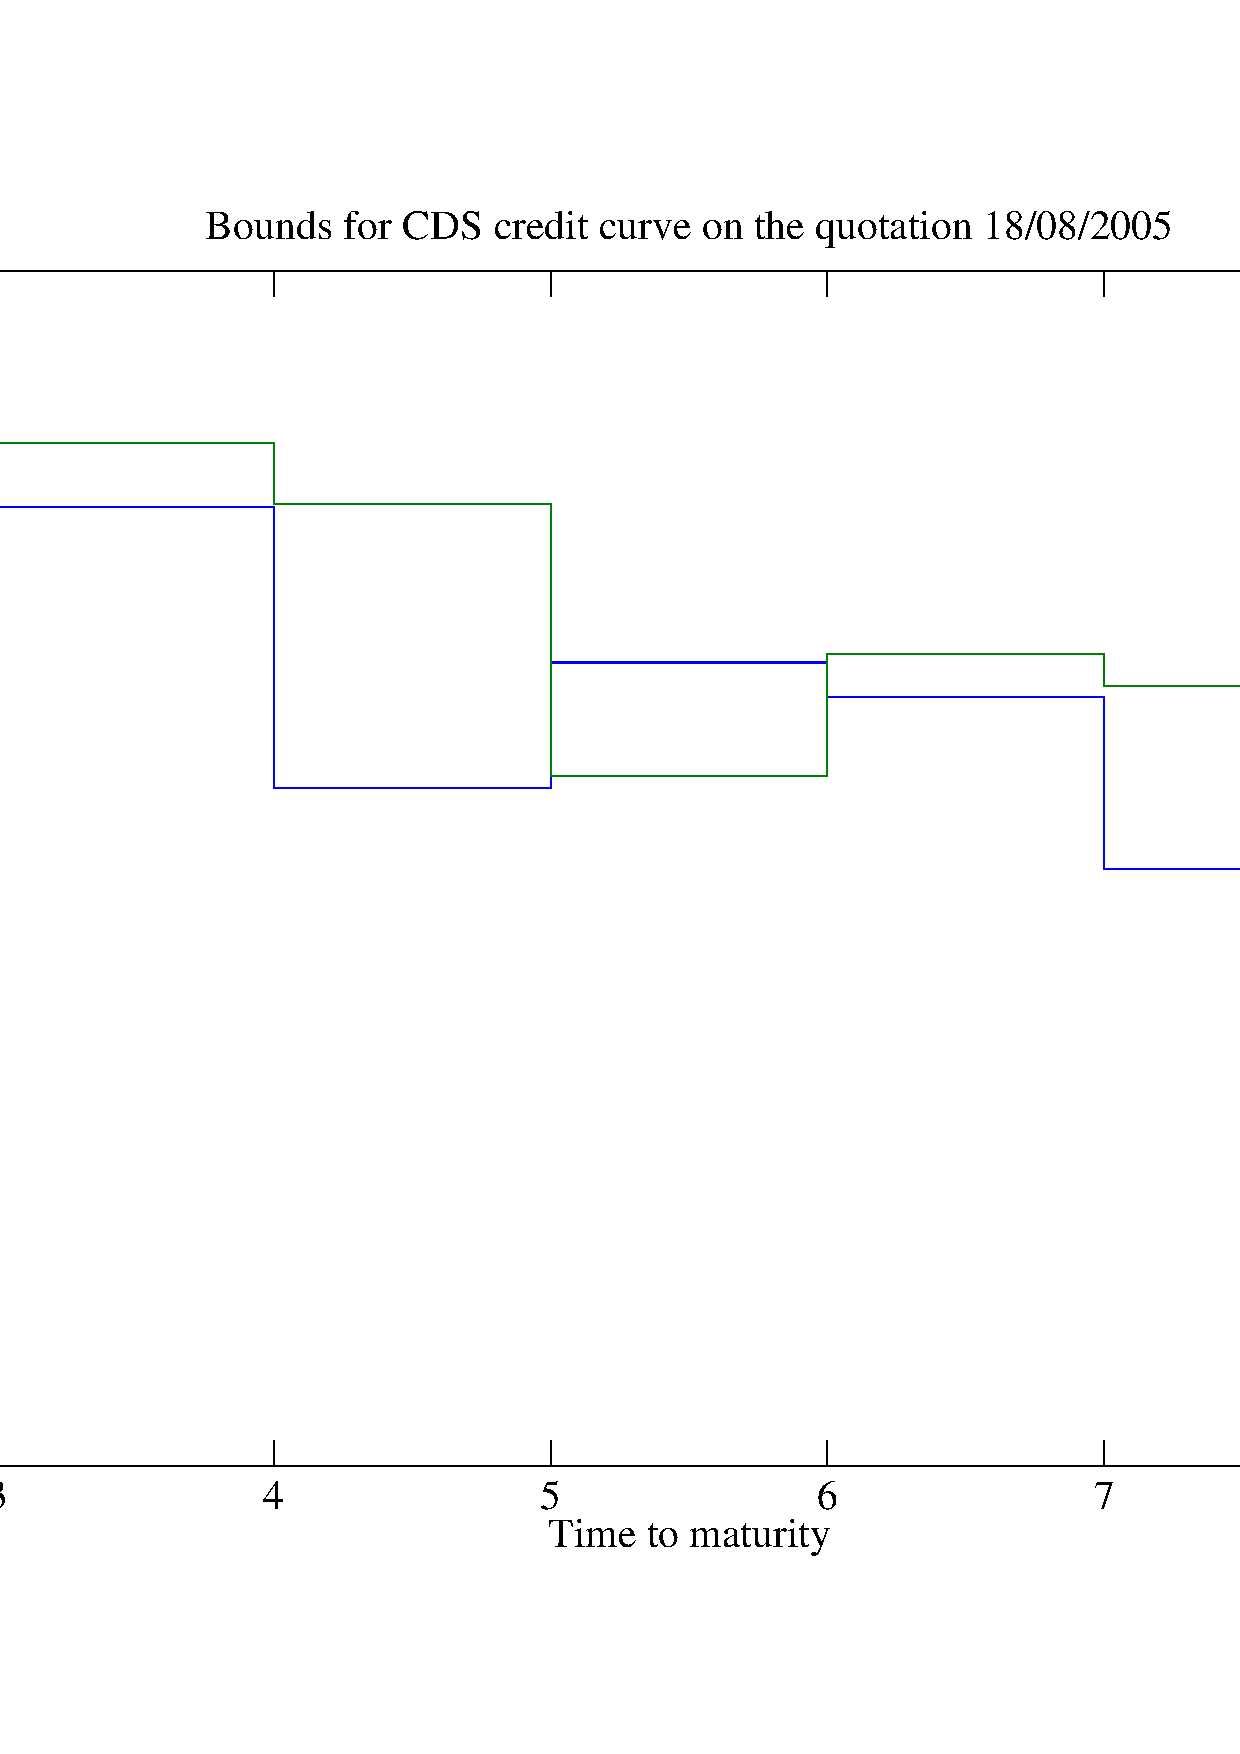
\includegraphics[width=0.8\textwidth]{cotation-18-08-2005.pdf}
  \caption{Credit curve among 18/08/2005 -  28/09/2007}
\end{figure}
\\
Since 28/09/2007 we can see that the credit curve fit well the market condition
:


\begin{figure}[H]
  \centering
  \includegraphics[width=0.8\textwidth]{cotation27-11-2007.pdf}
  \caption{Credit curve since 28/09/2007 : here in 27/11/2007}
\end{figure}

This is due to the lake of liquidity.\\
Let's remark that all curves must go through the gap defined at $T_i$ by
 $Qmax(T_{i})-Qmin(T_{i-1})$ :
 \begin{center}
   \begin{tikzpicture}
     \coordinate  (a) at  (0,1); \coordinate  (b) at  (1,1); \coordinate  (c) at
     (1,0.3);  \coordinate   (d)  at   (2,0.3);  \coordinate  (e)   at  (2,1.3);
     \coordinate (f)  at (1,1.3); \coordinate  (g) at (1,2); \coordinate  (h) at
     (0,2);

     \draw[color=blue]   (a)    --   (b);   \draw[color=blue]   (b)    --   (c);
     \draw[color=blue]   (c)    --   (d);   \draw[color=blue]   (d)    --   (e);
     \draw[color=blue]   (e)    --   (f);   \draw[color=blue]   (f)    --   (g);
     \draw[color=blue]   (g)    --   (h);   \draw[color=blue]   (h)    --   (a);
     \draw[color=red] (b) -- (f); \draw[color=red,->] (2,2) -- ($(b)!0.5!(f)$) ;
     \draw (2.2,2.2) node {gap}; \draw (h) .. controls (b) and (f) .. (d);

   \end{tikzpicture}

 \end{center}

In a  crisis period,  the company  will naturally  increase her  spreads values,
because the risk of illequidity will  increase. The company will be more mefiant
that of the entities that insure them and will impose a higher spreads value.

